%%%%%%%%%%%%%%%%%%%%%%%%%%%%%%%%%%%%%%%%%
% Structured General Purpose Assignment
% LaTeX Template
%
% This template has been downloaded from:
% http://www.latextemplates.com
%
% Original author:
% Ted Pavlic (http://www.tedpavlic.com)
%
% Note:
% The \lipsum[#] commands throughout this template generate dummy text
% to fill the template out. These commands should all be removed when 
% writing assignment content.
%
%%%%%%%%%%%%%%%%%%%%%%%%%%%%%%%%%%%%%%%%%

%----------------------------------------------------------------------------------------
%       PACKAGES AND OTHER DOCUMENT CONFIGURATIONS
%----------------------------------------------------------------------------------------

\documentclass{article}

\usepackage{fancyhdr} % Required for custom headers
\usepackage{extramarks} % Required for headers and footers
\usepackage{graphicx} % Required to insert images
\usepackage{enumerate}
\usepackage{amsmath}
\usepackage{comment}

% Margins
\topmargin=-0.45in
\evensidemargin=0in
\oddsidemargin=0in
\textwidth=6.5in
\textheight=9.0in
\headsep=0.25in 

\linespread{1.1} % Line spacing

% Set up the header and footer
\pagestyle{fancy}
\lhead{Linear Algebra with Application\\
to Engineering Computation}
\chead{}
\rhead{CME 200/ME300A\\
M. Gerristen\\
Fall 2013}
\headheight = 40pt

\renewcommand\headrulewidth{0.4pt} % Size of the header rule
\renewcommand\footrulewidth{0.4pt} % Size of the footer rule

\setlength\parindent{0pt} % Removes all indentation from paragraphs

%Add useful short-cut commands here

%1st order derivative wrt x
\newcommand{\dxone}[1]{\frac{d#1}{dx}}
%2nd order derivative wrt x
\newcommand{\dxtwo}[1]{\frac{d^2#1}{dx^2}}
%th in the exponent (e.g. when writing ith, instead use i$\eth$)
\newcommand{\eth}{^{\text{th}}}

%short-cuts for Greek letters
\newcommand{\al}{\alpha}
\newcommand{\dlt}{\delta}
\newcommand{\eps}{\epsilon}

%inverse
\newcommand{\inv}{^{-1}}
%cond
\newcommand{\cond}{\mathrm{cond}}
%trace
\newcommand{\trace}{\mathrm{trace}}

\newcommand{\twith}{\text{ with }}
\newcommand{\tand}{\text{ and }}
\newcommand{\tfor}{\text{ for }}

\newcommand{\ip}{_{i+1}}
\newcommand{\im}{_{i-1}}

\newcommand{\half}{\frac{1}{2}}
\newcommand{\oneby}[1]{\frac{1}{#1}}
\newcommand{\overto}[1]{\overset{#1}{\longrightarrow}}
%----------------------------------------------------------------------------------------
%       DOCUMENT STRUCTURE COMMANDS
%       Skip this unless you know what you're doing
%----------------------------------------------------------------------------------------

% Header and footer for when a page split occurs within a problem environment
\newcommand{\enterProblemHeader}[1]{
\nobreak\extramarks{#1}{#1 continued on next page\ldots}\nobreak
\nobreak\extramarks{#1 (continued)}{#1 continued on next page\ldots}\nobreak
}

% Header and footer for when a page split occurs between problem environments
\newcommand{\exitProblemHeader}[1]{
\nobreak\extramarks{#1 (continued)}{#1 continued on next page\ldots}\nobreak
\nobreak\extramarks{#1}{}\nobreak
}

\setcounter{secnumdepth}{0} % Removes default section numbers
\newcounter{homeworkProblemCounter} % Creates a counter to keep track of the number of problems

\newcommand{\homeworkProblemName}{}
\newenvironment{homeworkProblem}[1][Problem \arabic{homeworkProblemCounter}]{ % Makes a new environment called homeworkProblem which takes 1 argument (custom name) but the default is "Problem #"
\stepcounter{homeworkProblemCounter} % Increase counter for number of problems
\renewcommand{\homeworkProblemName}{#1} % Assign \homeworkProblemName the name of the problem
\section{\homeworkProblemName} % Make a section in the document with the custom problem count
\enterProblemHeader{\homeworkProblemName} % Header and footer within the environment
}{
\exitProblemHeader{\homeworkProblemName} % Header and footer after the environment
}
\newcommand\overmat[2]{%
  \makebox[0pt][l]{$\smash{\overbrace{\phantom{%
    \begin{matrix}#2\end{matrix}}}^{\text{$#1$}}}$}#2}

\newcommand{\problemAnswer}[1]{ % Defines the problem answer command with the content as the only argument
\noindent\framebox[\columnwidth][c]{\begin{minipage}{0.98\columnwidth}#1\end{minipage}} % Makes the box around the problem answer and puts the content inside
}

\title{Assignment 2 - Solutions}
\date{Issued: October 2, 2013}
\author{Due: October 9, in class\\
No late assignments accepted}

%----------------------------------------------------------------------------------------

\begin{document}

\maketitle
\thispagestyle{fancy}

%Problem 1
\begin{homeworkProblem}

\vspace{.5cm}
\begin{enumerate}[(a)]
%1(a)
\item In one dimension with $f(x) = 0$ and boundary conditions $T = 0$ at $x = 0$ and $T = 2$ at $x = 1$ we are solving the differential equation
\begin{equation} \dxtwo{T}=0\ \text{ with }\ T(0)=0,\ \ T(1) = 2. \end{equation}
The solution to this differential equation is a line of the form $T(x) = ax + b$. Setting $T=0$ at $x = 0$ we must have that $b = 0$. Setting $T = 2$ at $x = 1$ we must have that $a = 2$.
Therefore, we know the exact solution is $T(x) = 2x$.

%1(b)
\item To discretize the one dimensional problem (1), we use a uniform grid on $[0, 1]$ of $N + 1$ points with spacing $h = 1/N$. Therefore, the $i\eth$ point has coordinate $x_i = ih$ for $i = 0, \dots, N$.
Note that in constructing our grid in this fashion, we have exactly $N-1$ unknowns. The points $x_0 = 0$ and $x_N = 1$ have values fixed by the boundary conditions.
We now use the finite central difference equation derived in class to approximate the second derivative of $T$ at a point $x_i$,
\[ f_i = \dxtwo{T}|_{x=x_i} \approx \frac{T\ip-2T_i+T\im}{h^2}. \]
Because $f_i = f(x_i ) = 0$, at each $i$ we have the equation
\begin{equation} T\ip - 2T_i + T\im = 0,\ \ 1\le i \le N-1, \end{equation}
where our unknowns are the $N-1$ values $T_1, \dots, T_{N-1}$.
We must consider the boundary conditions $T(0) = T_0 = 0$ and $T(1) = T_N = 2$. The left boundary condition yields
\[ 0 = T_0 - 2T_1 + T_2 \implies 0 = -2T_1 + T_2. \]
The right boundary condition yields
\[ 0 = T_{N-2} - 2T_{N-1} + T_N \implies -2 = T_{N-2} - 2T_{N-1}. \]
We rewrite these equations in a more revealing form
\begin{equation}
\begin{matrix}
-2T_1 & + 1T_2 & & &                    & = 0\\
+1T_1 &- 2T_2 &+ 1T_3 & &       & = 0\\
 & +1T_2 &- 2T_3 &+ 1T_4 &      & = 0\\
 & & \vdots     & &                     & \vdots         \\
 & & +1T_{N-3} &- 2T_{N-2} &+ 1T_{N-1} & = 0\\
 & & & +1T_{N-2} &- 2T_{N-1}    & = -2
\end{matrix}
\end{equation}
Therefore, we see that $(1)$ gives us a system
\begin{equation}
\begin{bmatrix}
 -2 & 1 & & & &         \\
 1 & -2 & 1 & &         \\
   & 1 & -2 & 1 &       \\
   & & \vdots   & &     \\
   & & 1 & -2 & 1       \\
   & & & 1 & -2         \\
\end{bmatrix}
\begin{bmatrix} T_1     \\ T_2 \\ T_3 \\ \vdots \\ T_{N-2}\\ T_{N-1}
\end{bmatrix} = 
\begin{bmatrix} 0       \\ 0 \\ 0 \\ \vdots \\ 0 \\ -2
\end{bmatrix}
\end{equation}

%1(c)
\item For $N=5$ we want to perform Gaussian Elimination to show that the matrix is non-singular.
\[
A = \begin{bmatrix}
 -2 & 1 & 0 & 0         \\
 1 & -2 & 1 & 0         \\
 0 & 1 & -2 & 1         \\
 0 & 0 & 1 & -2                 \\
\end{bmatrix}\]
\[
\begin{bmatrix}
 -2 & 1 & 0 & 0         \\
 1 & -2 & 1 & 0         \\
 0 & 1 & -2 & 1         \\
 0 & 0 & 1 & -2                 \\
\end{bmatrix} \overto{R_2 \to R_2 + \half R_1}
\begin{bmatrix}
 -2 & 1 & 0 & 0         \\
 0 & -3/2 & 1 & 0               \\
 0 & 1 & -2 & 1         \\
 0 & 0 & 1 & -2                 \\
\end{bmatrix}
\overto{R_3 \to R_3 + \frac{2}{3} R_2}
\begin{bmatrix}
 -2 & 1 & 0 & 0         \\
 0 & -3/2 & 1 & 0               \\
 0 & 0 & -4/3 & 1               \\
 0 & 0 & 1 & -2                 \\
\end{bmatrix}
\]
\[
\overto{R_4\to R_4 + \frac{3}{4} R_3}
\begin{bmatrix}
 -2 & 1 & 0 & 0         \\
 0 & -3/2 & 1 & 0       \\
 0 & 0 & -4/3 & 1       \\
 0 & 0 & 0 & -5/4       \\
\end{bmatrix} \]
We see that we encounter no zero pivots. Hence the matrix A is nonsingular.

%1(d)
\item We want to show that $T(x)$, defined by
\[ T(x) = (2 + 40/(9\pi^2))x + 40/(9\pi^2)\sin(3\pi x/2), \]
satisfies the differential equation
\[\dxtwo{T} = -10\sin(3\pi x/2)\ \twith T(0)=0 \tand T(1) = 2. \]
Differentiating $T(x)$ twice we have
\[ T'(x) = 2 + 40/(9\pi^2) + 20/(3\pi) \cos(3\pi x/2), \]
\[ T''(x) = -10 \sin(3\pi x/2) = f (x). \]
Now checking the boundary conditions
\[ T(0) = (2 + 40/(9\pi^2))x + 40/(9\pi^2)\sin(3\pi x/2)|_{x=0} = 0 \]
\[ T(1) = (2 + 40/(9\pi^2)) + 40/(9\pi^2)\sin(3\pi/2) = 2 \]
We now construct and solve this system of equations in MATLAB using the following function that takes a parameter $n$ controlling the accuracy of the discretization:
\begin{verbatim}
function [T, x, A] = heatEqnSolver1D(N, f)
% This function solves the one dimensional Heat equation with Dirichlet boundary
% conditions T(0)=0 and T(1)=2 and returns two arrays, T and x.

% Inputs:
%    N:  controls the number of points in discretization with h = 1/N
%    f:  MATLAB function that evaluates the source function

% Find the points of discretization
h = 1/N;    % Interval size of discretization
x = 0:h:1;  % x = [x_0, x_1, ..., x_N]
x = x(2:end-1);  % x = [x_1, x_2, ..., x_{N-1}]

% Construct the tri-diagonal matrix A
A = diag(ones(N-2,1),1) - 2*eye(N-1) + diag(ones(N-2,1),-1);

% Instead of the line above, use the line below to take advantage of the sparsity of A.
% We can construct A as a sparse matrix directly (this will save us some memory space 
% and speed up computation)
% A = spdiags(ones(N-1,2), [-1;1], N-1, N-1) - 2*speye(N-1);

% Construct the right-hand side b from the function f
b = h^2*f(x)';
% Modify b to satisfy the Dirichlet boundary conditions
b(1) = b(1) - 0;     % Apply T_0 = 0
b(end) = b(end) - 2; % Apply T_N = 2

%Solve the system and return the result
T = A\b;
T = [0; T; 2];   % Reattach boundary values on T
x = [0; x'; 1];  % Reattach boundary values on x
end
\end{verbatim}

Now we solve for various $n$ and plot all of the results with the following commands:
\begin{verbatim}
% Run the following commands in MATLAB prompt
f = @(x) -10*sin(3*pi*x/2);
[T5, x5] = heatEqnSolver1D(5, f);
[T10, x10] = heatEqnSolver1D(10, f);
[T25, x25] = heatEqnSolver1D(25, f);
[T200, x200] = heatEqnSolver1D(200, f);
plot(x5, T5, x10, T10, x25, T25, x200, T200);
legend({'N=5', 'N=10', 'N=25', 'N=200'}, 'Location', 'NorthWest');
\end{verbatim}

These results are shown in Figure 1.

\begin{figure}[ht!]
\centering
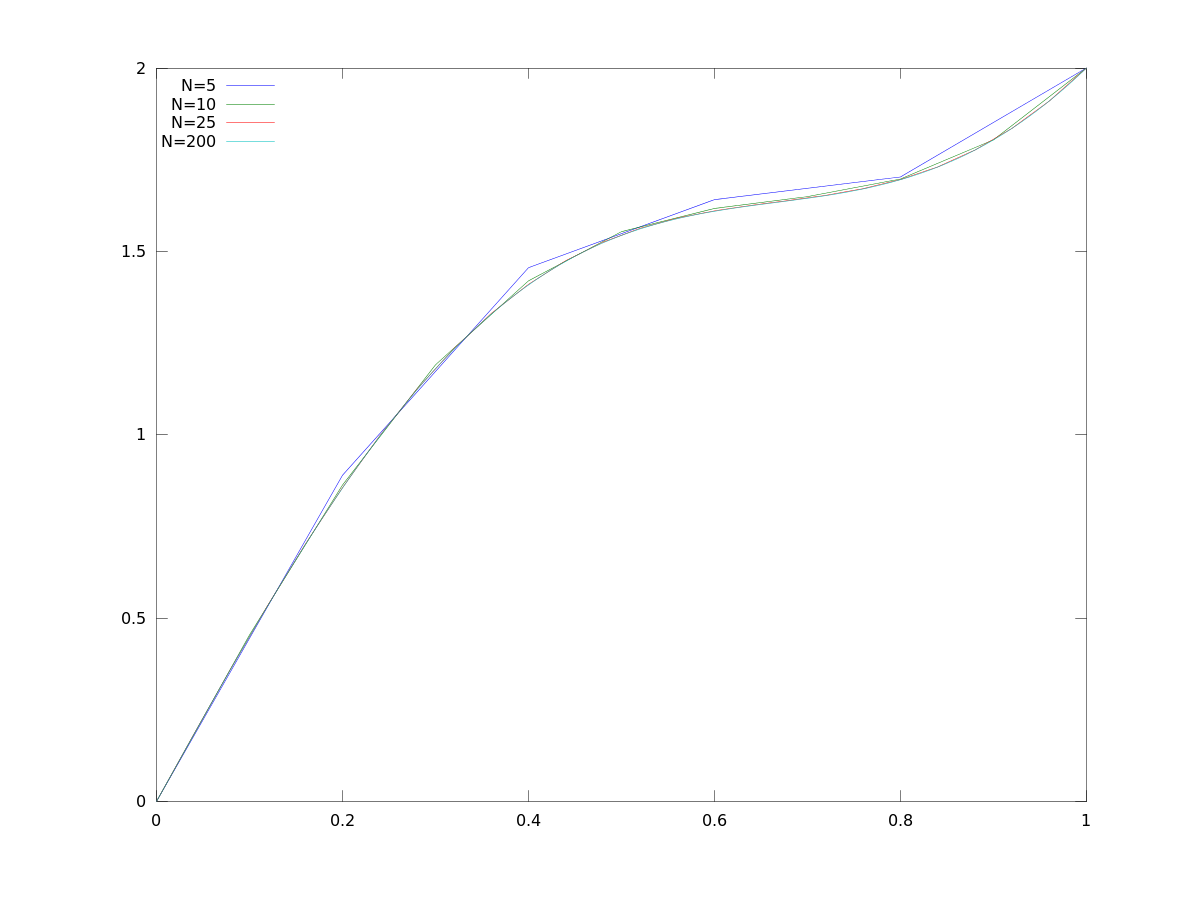
\includegraphics[width=1\linewidth]{1dheat.png}
\caption{1(d). Solution to the 1D heat equation with $f(x)=-10\sin(3\pi x/2)$ and boundary conditions $T(0)=0 \tand T(1)=2$.}
\label{fig:test}
\end{figure}

\newpage
%1(e)
\item We use the following MATLAB code to compute the condition number of the matrix $A \tfor N=5,\ N=10,\ N=25, \tand N=200$.

\begin{verbatim}
N = [5; 10; 25; 200]
cond_numbers = zeros(4, 1);
figure(2);
delta = 0.1;
f = @(x) -10*sin(3*pi*x/2);

c = ['r', 'b', 'k', 'g'];   % colors for plotting solution
for k=1:length(N)
  h = 1/(N(k));
% Construct sparse matrix A
  A = spdiags(ones(N(k)-1,2), [-1;1], N(k)-1, N(k)-1) - 2*speye(N(k)-1);

  A = A + delta*A;   % Perturbing the system by delta*A
  x = linspace(0, 1, N(k)+1);  % Find the points of discretization
  xind = x(2:end-1);
  b1 = (h^2)*(f(xind)); % Forming b
  b1(N(k)-1) = b1(N(k)-1) - 2;
  T = A\(b1');    % Solving the system Ax = b
  Tsol = [0; T; 2];

  plot(x', Tsol, c(k));
  hold on
  cond_numbers(k) = cond(A,'fro');   % Frobenius norm condition number
end

% Display condition numbers
cond_numbers
%{
   1.2931e+01
   7.6943e+01
   7.8663e+02
   1.4558e+05
%}

legend({'N=5', 'N=10', 'N=25', 'N=200'}, 'Location', 'SouthEast')
hold off

figure(3);
plot(cond_numbers);
\end{verbatim}

\begin{figure}[ht!]
\centering
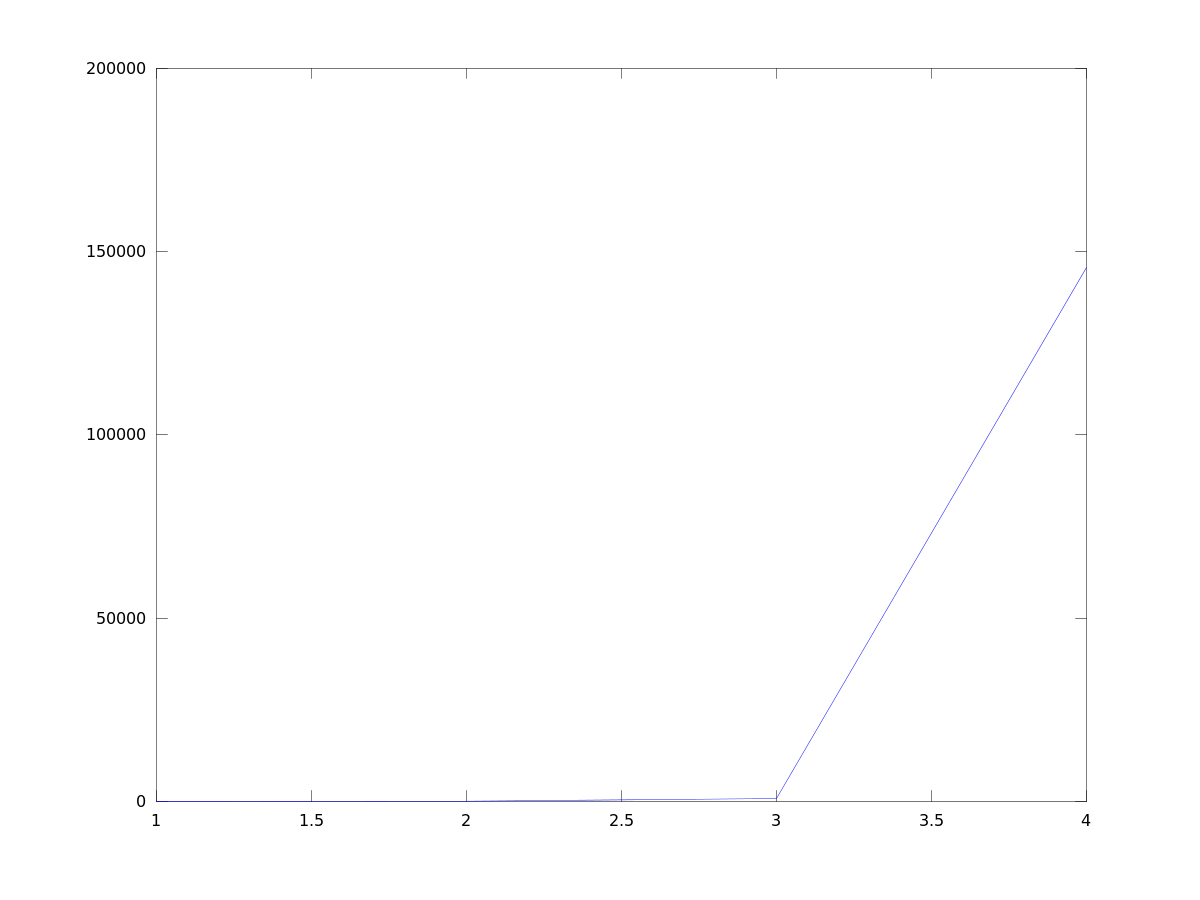
\includegraphics[width=.6\linewidth]{cond_numbers.png}
\caption{1(e). Variation of condition number with $N$.}
\label{fig:test}
\end{figure}

In Figure 2, we see that the condition number increases with $N$. The rate of increase is greater than 1 and depends on which norm is used to define the condition number (remember that $\cond(A) = \|A\|\|A\inv\|$). Intuitively, this should make sense since with greater number of points of discretization we should be able to notice perturbations to the system better.

\begin{figure}[ht!]
\centering
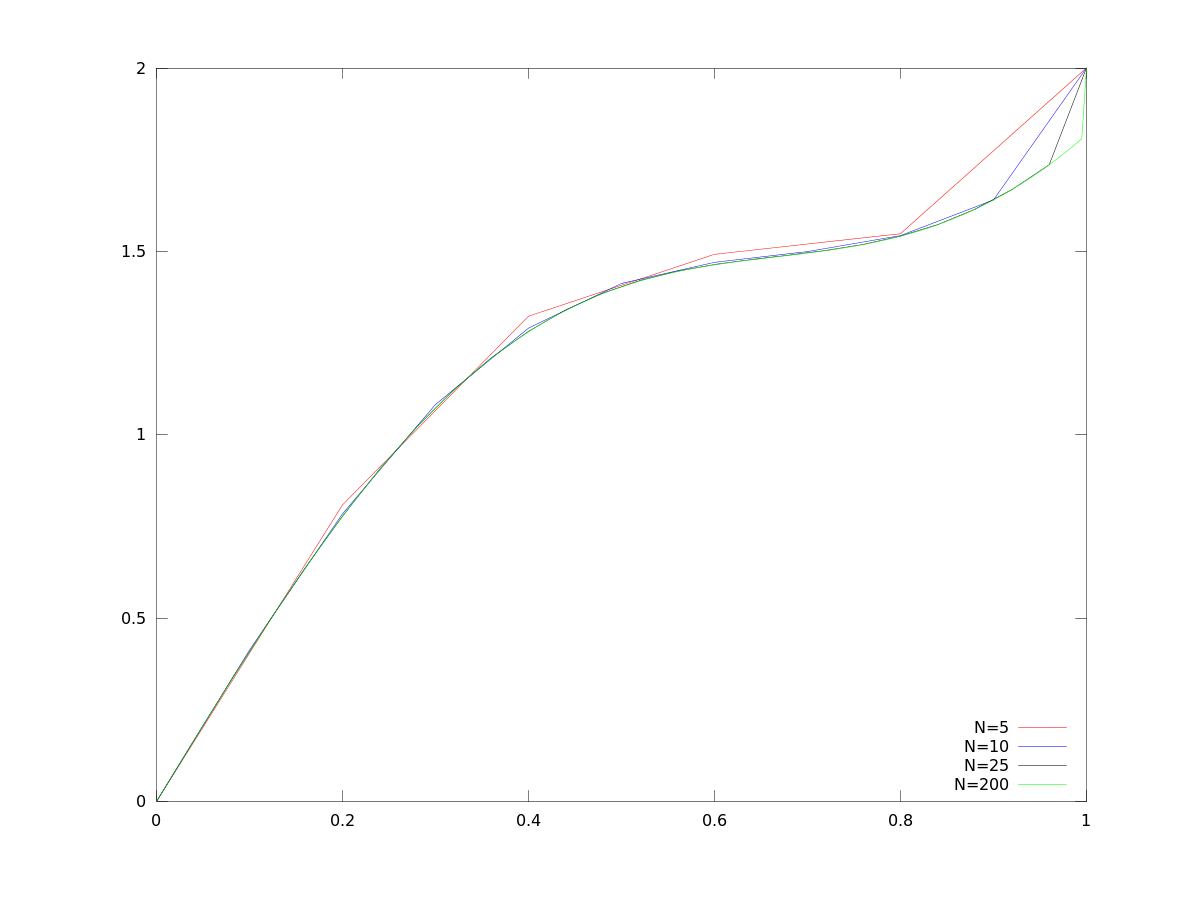
\includegraphics[width=.8\linewidth]{perturbed_sol.png}
\caption{1(e). Solution to the {\bf uniformly} perturbed system $(A + \partial{A})T = b$ for different values of $N$.}
\label{fig:test}
\end{figure}

\begin{figure}[ht!]
\centering
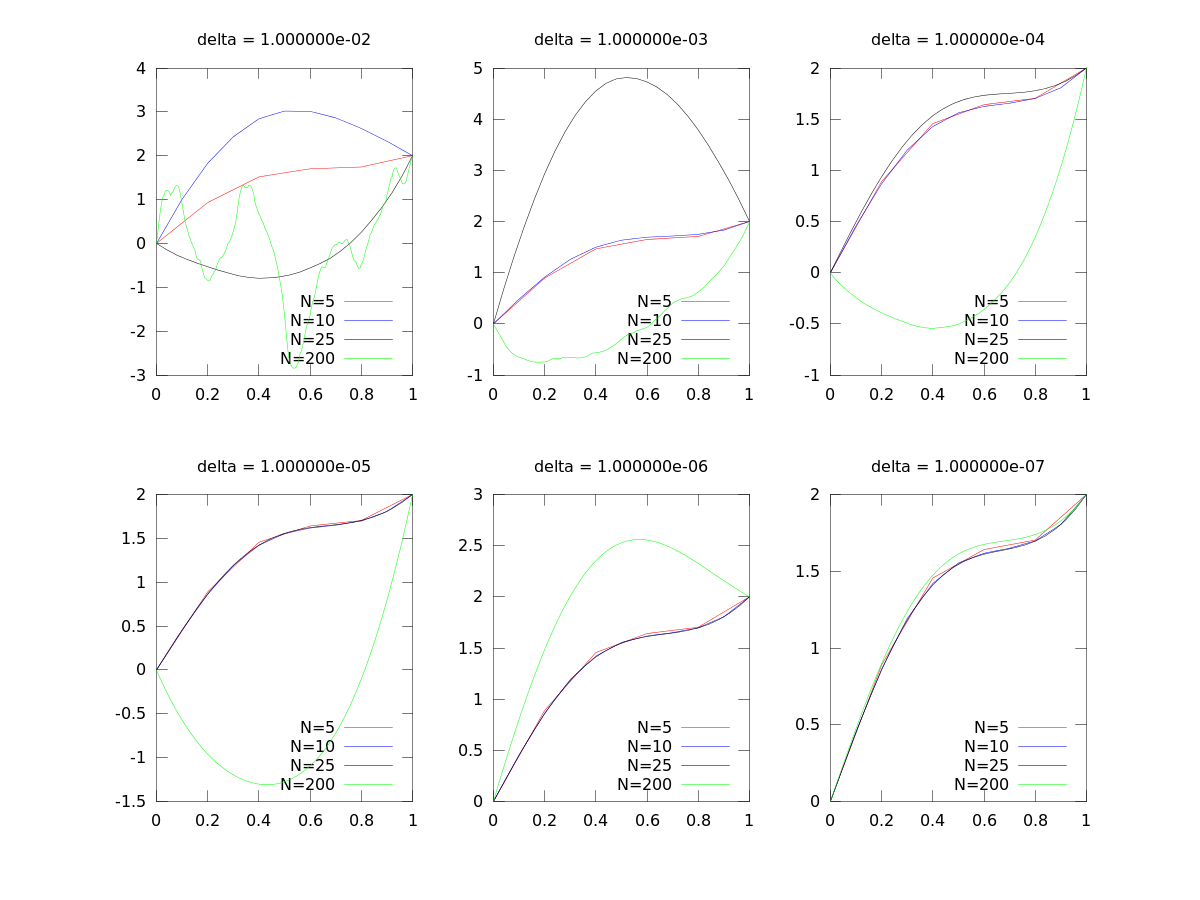
\includegraphics[width=.8\linewidth]{part_e_rand.png}
\caption{1(e). Solution to the {\bf randomly} perturbed system $(A + \partial{R})T = b$ for different values of delta.}
\label{fig:test}
\end{figure}

Although we see that the condition number is very large for N=200 case, the plot in Figure 3 does not show large changes to the solution as one could expect. However, keep in mind that the condition number only tells us the worst case performance. On the other hand if you use random perturbations as in,
\begin{verbatim}
  R = rand(N(i)-1,N(i)-1);
  A = A + delta*R;   % Perturbing the system by a random perturbation delta*R
\end{verbatim}
and let delta vary across a range of values, then you will observe that the solution produced by the discretization with N=200 grid points has the most volatile behaviour. The plot in Figure 4 shows the solutions resulted from 6 different values of delta.

%1(f)
\item We are given the equation $d^2T /dx^2 = f(x)$ with the boundary conditions $T=0$ at $x=0$ and $T=2$ at $x=1$ and the source function $f(x)$ defined piecewise 
\[ f(x) =   \left \{ \begin{array}{cc}  0 &  x < 1/3  \\ 100 & \text{otherwise.}  \end{array}  \right. \]
We want to verify that the exact solution to this differential equation is given by
\[ T(x) =   \left \{ \begin{array}{cc}  -\frac{182x}{9} &  x < 1/3  \\ \frac{-482x +50}{9} +\frac{100x^2}{2}  & \text{otherwise.}  \end{array}  \right. \]
We first check that the boundary conditions are satisfied:
\[ T(0) = -\frac{182\cdot 0}{9} = 0\ \tand\ T(1) = \frac{-482 + 50}{9} +\frac{100}{2} = -48 + 50 = 2. \]
We now verify that the solution is continuous by checking that the piecewise definition agrees at end point:
\[ T_1(1/3) = -\frac{182\cdot 1/3}{9} = -\frac{182}{27}, \]
\[ T_2(1/3) = \frac{-482/3 + 50}{9} +\frac{50}{9} = \frac{-482}{27} +\frac{100}{9} = -\frac{182}{27} = T_1(1/3). \]
Thus, $T(x)$ is indeed an exact solution of our differential equation.

Because of the way that we constructed the function heatEqnSolver1D, it is very easy to change the source term and get the plots. The only issue here is to compute the function $f$
to match the piecewise defined source function in the problem:
\begin{verbatim}
% Run these commands in MATLAB prompt window

% Exact solution
T = @(x) (-182/9*x)*(x<1/3) + ((-482*x+50)/9+50*x^2)*(x>=1/3);

x=0:0.01:1;
for k=1:length(x)
        t(k) = T(x(k));    % evaluate exact solution (for plotting)
end

f = @(x) 100*(x>1/3);

% Compute finite difference solutions
[T5, x5] = heatEqnSolver1D(5, f);
[T10, x10] = heatEqnSolver1D(10, f);
[T25, x25] = heatEqnSolver1D(25, f);
[T200, x200] = heatEqnSolver1D(200, f);

% Plot all solutions together
figure(1);
plot(x5, T5, x10, T10, x25, T25, x200, T200, x, t);
legend({'N=5', 'N=10', 'N=25', 'N=200', 'exact'}, 'Location', 'NorthWest');
\end{verbatim}

\begin{figure}[ht!]
\centering
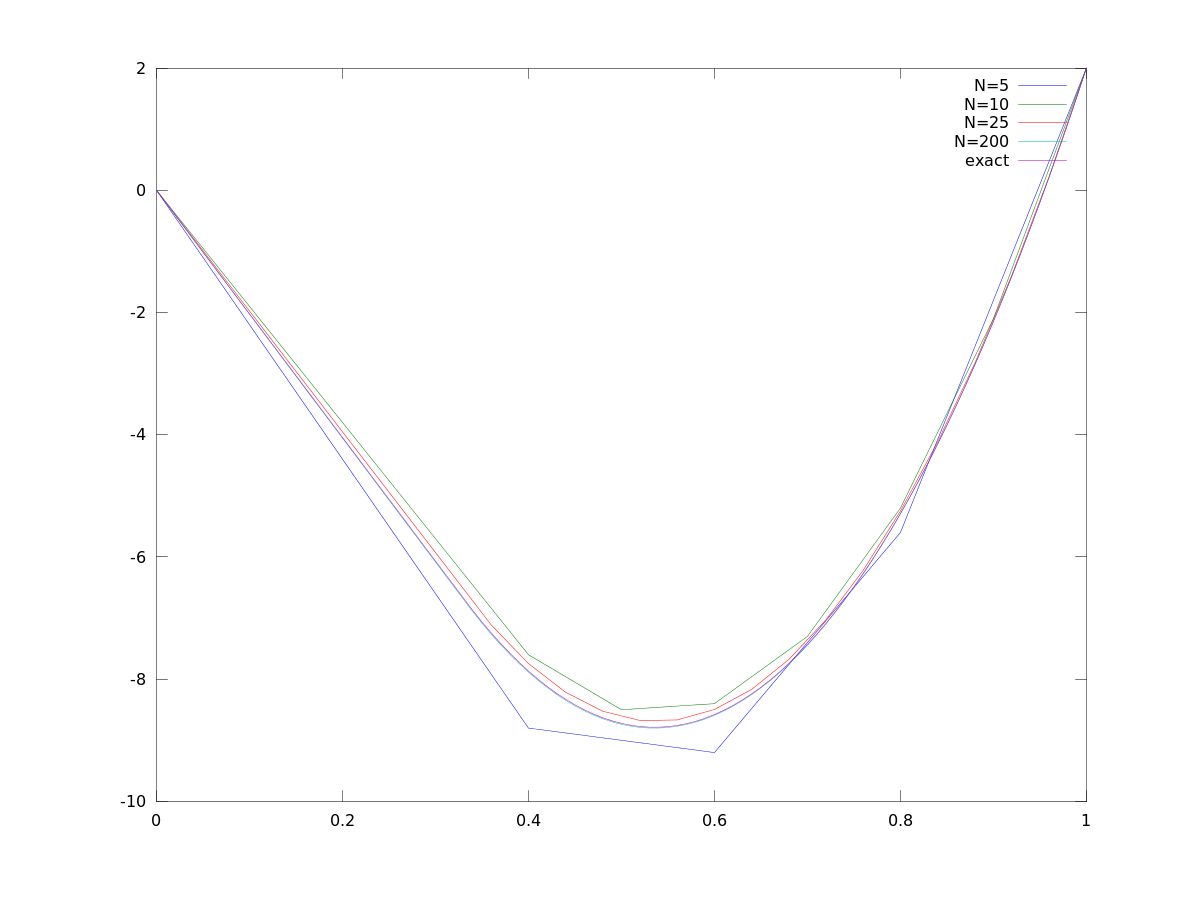
\includegraphics[width=.7\linewidth]{sol_part_f.png}
\caption{1(f). Solution to the 1D heat equation in part f.}
\label{fig:test}
\end{figure}

We now compute the relative error:
\begin{verbatim}
T_all = {T5, T10, T25, T200};  % cell array with all FD solutions
N = [5, 10, 25, 200];          % number of points used in discretizations
norms_exct = zeros(1,length(N));
rel_errors = zeros(1,length(N));

%compute relative errors wrt 2-norms
for m = 1:length(N)
  h = 1/N(m);       % Interval size of discretization
  x = 0:h:1;
  t = zeros(N(m),1);      % Initialize t (exact solution evaluated at N discrete locations)
  for k = 1:length(x)
    t(k) = T(x(k));
  end
  norms_exct(m) = norm(t);
  norms_exct_apprx(m) = norm(t - T_all{1,m});
  rel_errors(m) = norms_exct_apprx(m)/norms_exct(m);
end

% Plot relative errors
figure(2);
plot(N, rel_errors);
rel_errors
%rel_errors = [ 0.0897809   0.0328390   0.0137688   0.0017977 ]
\end{verbatim}

\begin{figure}[ht!]
\centering
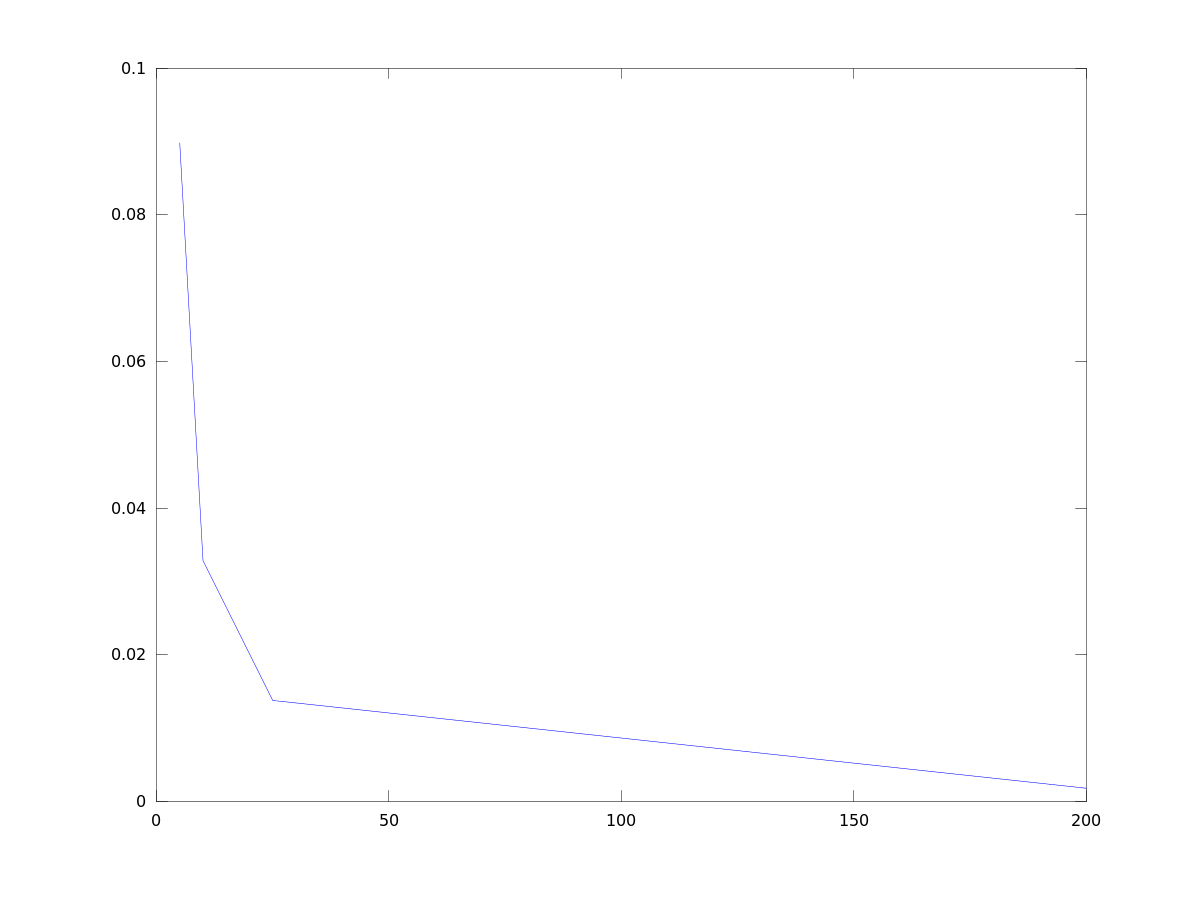
\includegraphics[width=.6\linewidth]{rel_errors.png}
\caption{1(f). Relative errors in part f.}
\label{fig:test}
\end{figure}

We now figure out how big does N have to be in order for the relative error to be less than 0.01. For that we first make a plot of all relative errors between 25 and 200 and observe an oscillatory exponential decrease in the errors (cf. Figure 7).
\begin{verbatim}
% Plot relative errors between 25 and 200
s=25;   % starting value of K
t=200;  % final value of K
rel_errs = zeros(1, t-s+1);
for K = s:t
  h = 1/K;    % Interval size of discretization
  x = 0:h:1;

  % compute exact solution evaluated at K discrete points
  T_exct = zeros(K,1);
  for k = 1:length(x)
    T_exct(k) = T(x(k));
  end
  norm_exct = norm(T_exct);

  %compute approx solution with FD discretization with K points
  [T_apprx, x5] = heatEqnSolver1D(K, f);

  %compute relative error
  norm_exct_apprx = norm(T_exct - T_apprx);
  rel_errs(K-s+1) = norm_exct_apprx/norm_exct;
end

figure(3);
plot([s:t],rel_errs);
\end{verbatim}
\begin{figure}[ht!]
\centering
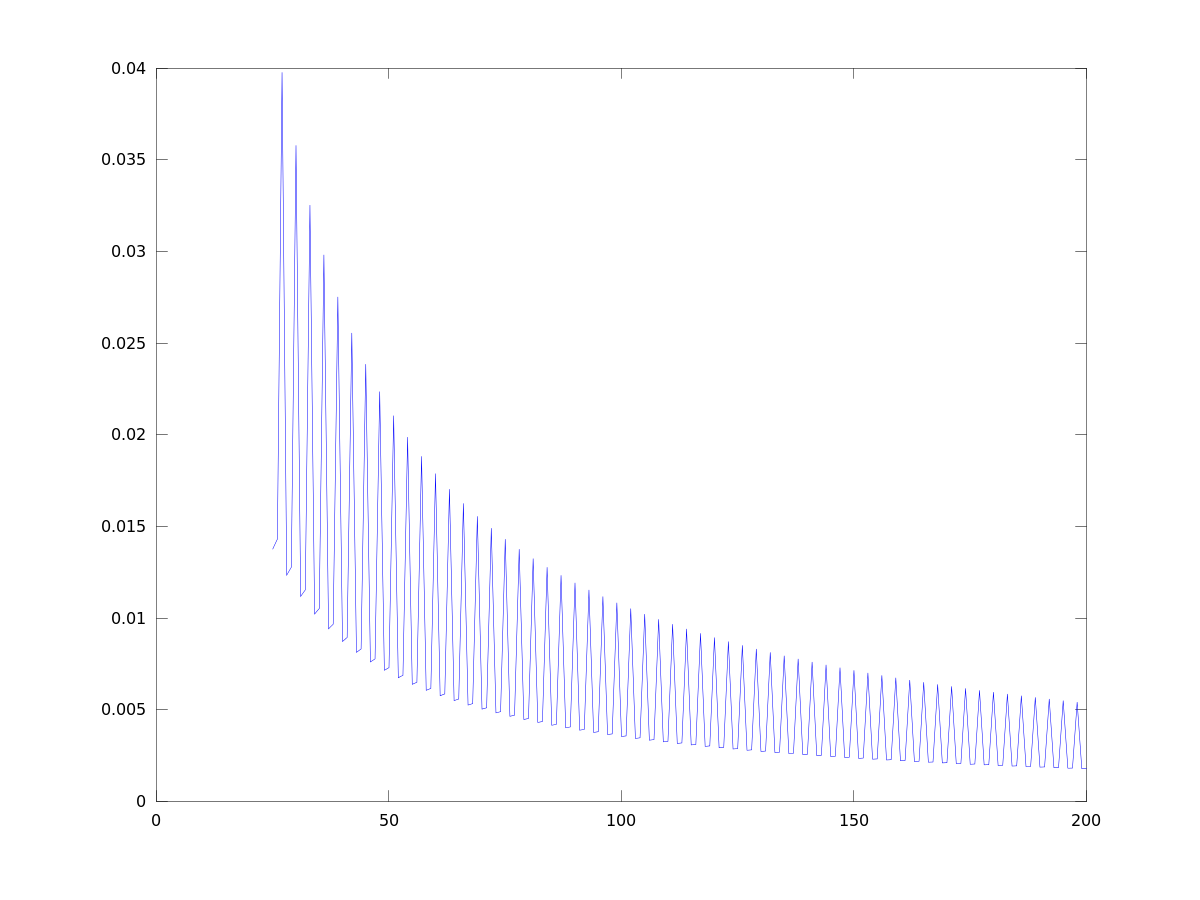
\includegraphics[width=.6\linewidth]{errors_partf.png}
\caption{1(f). Relative errors between $N=25$ and $N=200$.}
\label{fig:test}
\end{figure}

If you "zoom in" the graph in Figure 7 by plotting over a few consecutive values of $N$ (not shown here), you will notice that there is pattern to the observed oscillations. The higher errors occur when the grid points fall close to or exactly on the discontinuity of the source $f(x)$. This can be explained intuitively as follows. Since the source function is not defined at the jump, we are essentially taking a guess of what to pick as the value of $f(x)$ at the discontinuity and this uncertainty results in higher fluctuations in the numerical solution.\\
Looking at the graph we see that the errors do not exceed 0.01 for N larger than 120. Using this observation, we compute the smallest N (using linear search backtracking) which assures that the relative error is no greater than 0.01.
\begin{verbatim}
% Now starting at K=120 (obtained by looking at the last plot),
% backtrack to find the smallest value of N that
% will assure the relative error is less than err
err = 0.01;
K = 120;
rel_err = rel_errs(K-s+1);
%we use a linear backtracking search

while (K>s)
  K = K - 1;
  if(err == rel_errs(K-s+1))
    break;
  elseif(err < rel_errs(K-s+1))
    K = K+1;
    break;
  end
end

%display the smallest K and the corresponding relative error
K
rel_err = rel_errs(K-s+1)
% K =  106
% rel_err =  0.0033432
\end{verbatim}

By varying the value of $N$ we established that $N$ has to be at least $106$ to get the relative error $\frac{\| T_{exact,N} - T_N \|_2}{\| T_{exact} \|_2}$ less than 0.01.\\

When a grid point appears exactly on a point of discontinuity of the source $f(x)$, there are a number of ways to deal with this situation. For example, we could take the average value of $f(x)$ at the jump, or we could take either the limiting value to the left or to the right of the jump (i.e. the value of $f(x)$ as $x$ approaches the discontinuity from the left or from the right). However, in general we would try to discretize our domain in a way that avoids the points of discontinuity. In cases where a discontinuity cannot be avoided, the approach we use typically depends on the application.

%1(g)
\item When we applied boundary conditions in part (b) we were seeking to solve the system of equations given in equation (1). Now we have to represent the Neumann boundary conditions:
\[ 0 = \dxone{T}|_{x=0} \approx \frac{T_1-T_0}{h}\ \tand 0 = \dxone{T}|_{x=1} \approx \frac{T_N-T_{N-1}}{h} \]
Indeed, we can see that these boundary conditions just constrain the values next to the boundaries
\[ T_0 = T_1 \tand T_N = T_{N-1}. \]
Thus, our equations are
\[ T\ip - 2T_i + T\im = h^2f_i\ \tfor 1 < i < N-1, \]
and when we substitute the boundary conditions, we obtain
\[ -T_1 + T_2 = h^2f_1\ \tand\ T_{N-2} - T_{N-1} = h^2f_{N-1}. \]
Thus, with source $f(x)=0$, the system we obtain is
\begin{equation}
\begin{bmatrix}
 -1 & 1 & & & &         \\
 1 & -2 & 1 & &         \\
   & 1 & -2 & 1 &       \\
   & & \vdots   & &     \\
   & & 1 & -2 & 1       \\
   & & & 1 & -1         \\
\end{bmatrix}
\begin{bmatrix} T_1     \\ T_2 \\ T_3 \\ \vdots \\ T_{N-2}\\ T_{N-1}
\end{bmatrix} = 
\begin{bmatrix} 0       \\ 0 \\ 0 \\ \vdots \\ 0 \\ 0
\end{bmatrix}
\end{equation}
We check the $N=5$ case to see if it is singular
\[ A =
\begin{bmatrix}
 -1 & 1 & 0 & 0         \\
 1 & -2 & 1 & 0         \\
 0 & 1 & -2 & 1         \\
 0 & 0 & 1 & -1                 
\end{bmatrix} \to
\begin{bmatrix}
 -1 & 1 & 0 & 0         \\
 0 & -1 & 1 & 0         \\
 0 & 1 & -2 & 1         \\
 0 & 0 & 1 & -1                 
\end{bmatrix} \to
\begin{bmatrix}
 -1 & 1 & 0 & 0         \\
 0 & -1 & 1 & 0         \\
 0 & 0 & -1 & 1         \\
 0 & 0 & 1 & -1                 
\end{bmatrix} \to
\begin{bmatrix}
 -1 & 1 & 0 & 0         \\
 0 & -1 & 1 & 0         \\
 0 & 0 & -1 & 1         \\
 0 & 0 & 0  & 0                 
\end{bmatrix} = U \]

The two systems, $A \vec x = \vec b$ and $U \vec x = \vec b$, have the same solutions. Since the last row of $U \vec x = \vec b$ is satisfied for any value of $\vec x$, it can be eliminated from the system without changing the solution. This leaves us with the system

\begin{equation}
\begin{bmatrix}
 -1 & 1 & 0 & 0         \\
 0 & -1 & 1 & 0         \\
 0 & 0 & -1 & 1          
\end{bmatrix}
\begin{bmatrix}
T_1  \\ T_2 \\ T_3 \\ T_4
 \end{bmatrix} =
 \begin{bmatrix}
 0 \\ 0 \\ 0
 \end{bmatrix}
\end{equation}

At last we can fix $T_4$ to any value $c$ (any other $T_i$ works as well)  to get the system\\
\begin{equation}
\begin{bmatrix}
 -1 & 1 & 0 &           \\
 0 & -1 & 1 &           \\
 0 & 0 & -1 &            
\end{bmatrix}
\begin{bmatrix}
T_1  \\ T_2 \\ T_3 \\ 
 \end{bmatrix} =
 \begin{bmatrix}
 0 \\ 0 \\ -c
 \end{bmatrix},
\end{equation}
which is easily seen to be solvable through back substitution.

%1(h)
\item Following the same methodology as in 1(b) and 1(g), we get the boundary conditions as
\[ T_0 = 0\ \tand\ T_N = T_{N-1}, \]
and we obtain the matrix-vector equation of the form,
\[ \begin{bmatrix}
-2 & 1 & & & &          \\
 1 & -2 & 1 & &         \\
   & 1 & -2 & 1 &       \\
   & & \vdots   & &     \\
   & & 1 & -2 & 1       \\
   & & & 1 & -1         
\end{bmatrix}
\begin{bmatrix} T_1     \\ T_2 \\ T_3 \\ \vdots \\ T_{N-2}\\ T_{N-1}
\end{bmatrix} = 
\begin{bmatrix} 0       \\ 0 \\ 0 \\ \vdots \\ 0 \\ 0
\end{bmatrix} \]
For $N=5$,
\[ A =
\begin{bmatrix}
 -2 & 1 & 0 & 0         \\
 1 & -2 & 1 & 0         \\
 0 & 1 & -2 & 1         \\
 0 & 0 & 1 & -1                 
\end{bmatrix} \]
$A$ is non-singular since $\det(A)\neq 0$.
\end{enumerate}
\end{homeworkProblem}

%Problem 2
\begin{homeworkProblem}
TRUE or FALSE.
\begin{enumerate}[(a)]
%2(a)
\item  $\trace(A^TA)=\|A\|_F$. True.
\\ Let $A = [\vec{a}_1\ \vec{a}_2\ \dots\ \vec{a}_n],$ where $\vec{a}_1,\ \vec{a}_2,\ \dots,\ \vec{a}_n$ are the columns of $A$.
\[ A^T = \begin{bmatrix} \vec{a}_1^T    \\ \vec{a}_2^T \\ \vdots \\ \vec{a}_n^T \end{bmatrix}\ \ \ \ \ \ \ \ \ \ 
 A^TA =
\begin{bmatrix}
 \vec{a}_1^T \vec{a}_1 & \vec{a}_1^T \vec{a}_2 & \dots & \vec{a}_1^T \vec{a}_n  \\
 \vec{a}_2^T \vec{a}_1 & \vec{a}_2^T \vec{a}_2 & \dots & \vec{a}_2^T \vec{a}_n  \\
   &   & \vdots &       \\
 \vec{a}_n^T \vec{a}_1 & \vec{a}_n^T \vec{a}_2 & \dots & \vec{a}_n^T \vec{a}_n  
\end{bmatrix} \]
$\trace(A^TA)=$ sum of the diagonal elements of $A^TA = 
\sum\limits_{i=1}^n \vec{a}_i^T \vec{a}_i = \sum\limits_{i=1}^n \sum\limits_{j=1}^n a_{ij}^2 = \|A\|_F$.

%2(b)
\item $\cond(\al A) = \al\ \cond(A)$. False.\\
$(\al A)\inv = \oneby{\al} A\inv$. 
Taking $\al>1$, we show that the statement above does not hold in general,
\[ \cond(\al A) = \|\al A\| \|(\al A)\inv\| = \al \|A\| \oneby{\al} \|A\inv\| = \|A\| \|A\inv\| = \cond(A) \neq \al\ \cond(A). \]

\end{enumerate}
\end{homeworkProblem}

\end{document}
